\documentclass[author-year, review]{elsarticle} %review=doublespace preprint=single 5p=2 column
%%% Begin My package additions %%%%%%%%%%%%%%%%%%%
\usepackage[hyphens]{url}
\usepackage{lineno} % add 
\bibliographystyle{elsarticle-harv}
\biboptions{sort&compress} % For natbib
\usepackage{graphicx}
\usepackage{booktabs} % book-quality tables
%% Redefines the elsarticle footer
\makeatletter
\def\ps@pprintTitle{%
 \let\@oddhead\@empty
 \let\@evenhead\@empty
 \def\@oddfoot{\it \hfill\today}%
 \let\@evenfoot\@oddfoot}
\makeatother

% A modified page layout
\textwidth 6.75in
\oddsidemargin -0.15in
\evensidemargin -0.15in
\textheight 9in
\topmargin -0.5in
%%%%%%%%%%%%%%%% end my additions to header

\usepackage[T1]{fontenc}
\usepackage{lmodern}
\usepackage{amssymb,amsmath}
\usepackage{ifxetex,ifluatex}
\usepackage{fixltx2e} % provides \textsubscript
% use upquote if available, for straight quotes in verbatim environments
\IfFileExists{upquote.sty}{\usepackage{upquote}}{}
\ifnum 0\ifxetex 1\fi\ifluatex 1\fi=0 % if pdftex
  \usepackage[utf8]{inputenc}
\else % if luatex or xelatex
  \usepackage{fontspec}
  \ifxetex
    \usepackage{xltxtra,xunicode}
  \fi
  \defaultfontfeatures{Mapping=tex-text,Scale=MatchLowercase}
  \newcommand{\euro}{€}
\fi
% use microtype if available
\IfFileExists{microtype.sty}{\usepackage{microtype}}{}
\usepackage{longtable}
\let\parencite\cite
\usepackage{graphicx}
% Redefine \includegraphics so that, unless explicit options are
% given, the image width will not exceed the width of the page.
% Images get their normal width if they fit onto the page, but
% are scaled down if they would overflow the margins.
\makeatletter
\def\ScaleIfNeeded{%
  \ifdim\Gin@nat@width>\linewidth
    \linewidth
  \else
    \Gin@nat@width
  \fi
}
\makeatother
\let\Oldincludegraphics\includegraphics
{%
 \catcode`\@=11\relax%
 \gdef\includegraphics{\@ifnextchar[{\Oldincludegraphics}{\Oldincludegraphics[width=\ScaleIfNeeded]}}%
}%

\makeatletter
\def\maxwidth{\ifdim\Gin@nat@width>\linewidth\linewidth\else\Gin@nat@width\fi}
\def\maxheight{\ifdim\Gin@nat@height>\textheight\textheight\else\Gin@nat@height\fi}
\makeatother
% Scale images if necessary, so that they will not overflow the page
% margins by default, and it is still possible to overwrite the defaults
% using explicit options in \includegraphics[width, height, ...]{}
\setkeys{Gin}{width=\maxwidth,height=\maxheight,keepaspectratio}

\renewcommand\includegraphics[2][]{%
    {\vspace{0.5cm}\centerline{\Oldincludegraphics[#1, width=\maxwidth, keepaspectratio]{#2}\\}\vspace{0.5cm}}
}

\ifxetex
  \usepackage[setpagesize=false, % page size defined by xetex
              unicode=false, % unicode breaks when used with xetex
              xetex]{hyperref}
\else
  \usepackage[unicode=true]{hyperref}
\fi
\hypersetup{breaklinks=true,
            bookmarks=true,
            pdfauthor={},
            pdftitle={NLP for political polarity classification from tweets},
            colorlinks=true,
            urlcolor=blue,
            linkcolor=magenta,
            pdfborder={0 0 0}}
\urlstyle{same}  % don't use monospace font for urls
\setlength{\parindent}{0pt}
\setlength{\parskip}{6pt plus 2pt minus 1pt}
\setlength{\emergencystretch}{3em}  % prevent overfull lines
\setcounter{secnumdepth}{5}
% Pandoc toggle for numbering sections (defaults to be off)
% Pandoc header
\protect\newcommand\nohyph{\hyphenpenalty=10000\relax\exhyphenpenalty=10000\relax}

\usepackage{mathtools}
\DeclarePairedDelimiter{\ceil}{\lceil}{\rceil}
\DeclarePairedDelimiter{\floor}{\lfloor}{\rfloor}
\DeclarePairedDelimiter\abs{\lvert}{\rvert}
\newcommand\tab[1][1cm]{\hspace*{#1}}
\usepackage{amsmath}
\usepackage{algorithm}
%\usepackage[noend]{algpseudocode}
\usepackage{algpseudocode}
\algnewcommand\algorithmicinput{\textbf{Input:}}
\algnewcommand\INPUT{\item[\algorithmicinput]}
\algnewcommand\algorithmicoutput{\textbf{Output:}}
\algnewcommand\OUTPUT{\item[\algorithmicoutput]}

\let\emptyset\varnothing

\algblockdefx[Foreach]{Foreach}{EndForeach}[1]{\textbf{for each} #1 \textbf{do}}{\textbf{end for}}
\algblockdefx[ParallelFor]{ParallelFor}{EndParallelFor}[1]{\textbf{parallel for} #1 \textbf{do}}{\textbf{end for}}
\makeatletter
\ifthenelse{\equal{\ALG@noend}{t}}{\algtext*{EndForeach}}{}
\ifthenelse{\equal{\ALG@noend}{t}}{\algtext*{EndParallelFor}}{}
\makeatother
\makeatletter
\def\BState{\State\hskip-\ALG@thistlm}
\makeatother

\usepackage{float}
\usepackage{capt-of}
\setlength{\parskip}{0pt}
\setlength{\parsep}{0pt}
\setlength{\headsep}{0pt}
\setlength{\topskip}{0pt}
\setlength{\topmargin}{0pt}
\setlength{\topsep}{0pt}
\setlength{\partopsep}{0pt}
\usepackage{cleveref}
\crefname{lstlisting}{listing}{listings}
\Crefname{lstlisting}{Listing}{Listings}



\begin{document}
\begin{frontmatter}

  \title{\protect\hypertarget{_Hlk498998102}{}{}NLP for political polarity
classification from tweets}
      \author{\protectNisim Jonatan Hurst Tarrab}
    
  \begin{abstract}
  Tweets are a common way for political candidates to pronounce themselves about some topic. However, the use of jargon, open ended language and lack of context turn most of the direct classification methods useless. However, cues of the political and twitter realm can be used to extract features that can improve sentiment analysis substantially. In this work we will follow mainly the approach proposed by \parencite{2002a} of using machine learning classifiers but also will in some way give a limited amount of importance to the gramatical structures. We first extract common sense features, that hereby are called \emph{special tokens}. Then, we merge those features with bigrams of special tokens that probably take precedence in each of the attitudes. Finally, word2vec attributes are used to compute sentence orientation regardless of word order. Word2vec features can preserve syntactical and semantical relationships between words. The main contribution of this work is to be a proof-of-concept for extracting syntactic grammatical and semantic features on the domain of actual Mexican policy that improve automatic tweet attitude tagging. A simple special tokens bigram counts and wrod2vec features have shown an improvement over bag-of-word of y on average and an improvement of 0.07 and 0.20 respectively.
  \end{abstract}
  
 \end{frontmatter}


\small


\section{Introduction and problem
understanding}\label{introduction-and-problem-understanding}

Tweets are a common way for political candidates to express their
opinions about current affairs. Since the arrival of the Web 2.0
microblogging platforms have become political instruments and reveal
political attitudes of political candidates all over the world (except
for those places in which government controls internet access like
China). An example of previous work done on the pollical milieu can be
found on
\parencite{2010},
\parencite{2011}
and
\parencite{22012}.

A group of Mexican anthropological researchers (Marta Bárbara Ochman et
al., 2016) took the task of making a taxonomy just for classifying
political attitudes that can be identified on tweets. Their hypothesis
is that those attitudes are correlated with future campaign proposals.
The taxonomy developed was the following:

\begin{enumerate}
\def\labelenumi{\arabic{enumi}.}
\item
  Proactive: Tweets under this category are aimed to generate
  information about their personal virtues, their proposed program and
  their party's current efforts.
\item
  Reactive: Seek to neutralize their adversaries' derisions and any
  infamous depiction on the media.
\item
  Aggressive: Emphasize negative traits of their enemies or defame their
  opponents.
\item
  Vote winner: Demagogue speech aimed at winning a political advantage.
\end{enumerate}

No one can gainsay that labeling each of these tweets is drudgery. Thus,
a model that can classify those tweets with minimal human intervention
is highly desirable.

However, this task isn't easy. Tweets are very limited in the following
ways
\parencite{12014}:

\begin{itemize}
\item
  Data sparsity.
\item
  Changing nature of languages due to trending topics.
\item
  Political candidates usually make use of jargon and informal language.
\item
  Lack of context from the text. The text field is limited to 40
  characters.
\item
  Short irregular forms may be used.
\end{itemize}

Clearly, if we try to use a machine learning classifier over the raw
tweets headfirst, the results would be disappointing. So, on the one had
we have these data highly skewed and sparse with the problems just
mentioned. On the other hand, we have all these mature machine learning
algorithms dating back to the 50's. We need to find good instance
representation that our models can use uniformly, expresses latent
attributes present in the data and finally reduce noise produced by
redundant features that just doesn't add any value. But how?.



\begin{figure}[H]

\label{fig:commontasks}

\centering

\begin{minipage}{\textwidth}



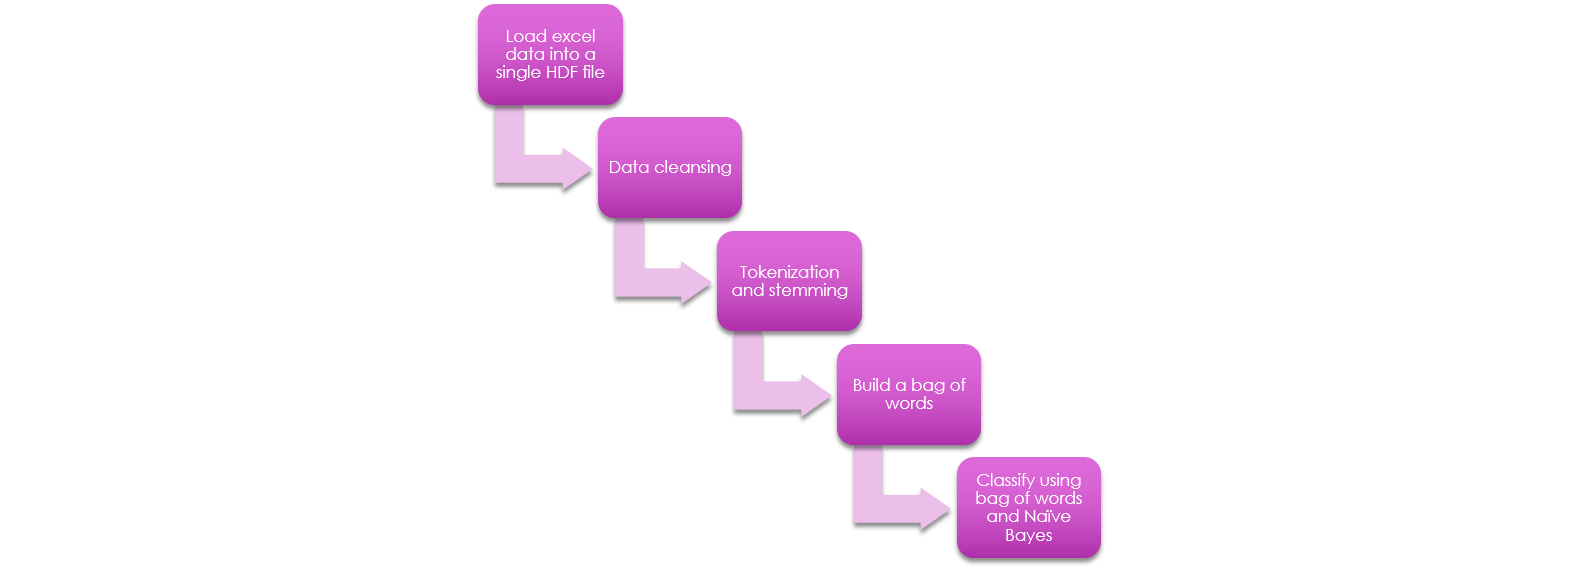
\includegraphics[width=6.49583in,height=2.33889in]{.//media/image1.png}



\end{minipage}

\caption{Text preprocessing pipeline}

\end{figure}



Well, firstly we should use some common preprocessing steps that might
help semantic and grammar decomposition or somehow incorporate domain
knowledge into our search space. These techniques are show in
\Cref{fig:commontasks}.
Secondly, deep learning techniques using CNN have prove to be useful in
many realms, from heuristics design to computer vision. NLP is not an
exception. Here we can used them to extract those latent features we
mentioned earlier. A common technique that has been infallible is
word2vec. Since its conception in
\parencite{2013},
this method has been capable of both preserving semantic and syntactic
representation and can be used reliably to categorize a bag-of-words
when data is sparse.

The initial hypothesis of the projects is:

\begin{enumerate}
\def\labelenumi{\arabic{enumi}.}
\item
  A set of features represented in a word2vec vector representation of
  the tweet can leverage the power of an already trained word2vec model
  and gives a Naïve Bayes classifier a very low generalization error
  \footnotemark\footnotetext{\nohyph Although there exists an Spanish corpus it is not focused on political jargon and each party has its own jargon}.
\item
  A more diverse set of features can increase accuracy
  \parencite{2018}.
  Thus, a minimum representation of a grammatical structure, i.e. a
  bigram count of \emph{special tokens} are added to the resulting set
  of features. This bigram count increases the classifiers accuracy.
\item
  Normalized features achieve better results and can be selected more
  easily because they are scale invariant. Thus, the vectors
  corresponding to tweets with different lengths are weighted. However,
  tweet length will be added to the features in representation of
  energetic grammatical structures.
\end{enumerate}

Results show that the ROC AUC curve increases significantly, from 0.65
(on average for the four political attitudes) using only bag of words to
0.72 using only bigram features, to 0.85 using word2vec features and
finally to 0.857 using all the features.

In the final model we will see that the top 5 most important features
are for all the four labels coming from V2W.

\section{Previous works}\label{previous-works}

\parencite{1--22008}
places Sentiment Analysis (SA) within the área of Natural Language
Processing (NLP) and can be defined as the computational treatment of
opinions, feelings, and subjectivity in text. This article mentions that
early history places 2001 as the milestone at which a widespread
awareness began to arise around sentiment analysis, with beliefs systems
as forerunners. One of the factors behind this land rush was the
availability of datasets for machine learning on the World Wide Web.

\parencite{12014}
brings to the table two of the firsts approaches for the research
community to tackle the problem of SA.
\parencite{2002b}
proposes the use of linguistic analysis. This kind of approach can be
thought as supervised because it relies on previous domain knowledge,
e.g. Chomsky grammatical structures. At the other end we have
\parencite{2002a},
which proposes the use of classical machine learning techniques.
Contrary to the approach taken by Turney, here we rely more on achieving
a high accuracy using an ensemble of different techniques, commonly
ignoring grammatical structures as in the case of a simplification using
bag-of-words representation.

The bag-of-words representations gets its name form a passage from
linguist Zellig Harris (1954), ``language is not merely a bag of words
but a tool with particular properties.''.
\parencite{2012}
suggest we think of the model as ``putting the words of the training
corpus'' in a bag and then selecting one word at a time. Then, the
notion of order is lost, but we end up with a binary vector that we can
neatly use in our machine learning classifiers.

Now, let's go back to a more recent 5-year horizon. As aforementioned
there is an extreme impairment over context in which we are just
fettered to a 140 characters text context. Furthermore, tweets usually
don't have representative and syntactically consistent words.
\parencite{102013}
proposes a sentiment grade for each distinct notion in the post using an
ontology instead of evaluating it as a whole. The authors use a
\emph{Formal Concept Analysis} (FCA) algorithm proposed by
\parencite{1999}
in which applies a user-driven-step-by-step methodology for creating
domain models, i.e. it creates an ontology specific for the bulk of
tweets to classified. Tweets were classified on a rank per topic. They
used a tool called OntoGen in which a semi-supervised approach was
possible.

Through the lens of our work, topic and ontologies could prove useful
when considering political parties, allies, government institutions,
commercial and foreign institutions. However, these ontologies must be
built mostly by human annotations, a cost we cannot afford in this
study.

The approach taken by
\parencite{42013}
was a bit different. The paper measures how to word of mouth (WOM)
affect movies sales, negatively or positively. There were four tweet
categories very similar to the ones we are measuring: intention tweets,
positive tweets, neutral tweets and negative tweets. \emph{Intention
tweets} are very similar to our \emph{vote winner} category because an
intention to win votes can be achieved either by aggressive of proactive
tweets. The authors decided to use two well-known classical machine
learning classifiers: Naïve Bayes and Support Vector Machines. This
approach is similar the one proposed by
\parencite{2002a}
in which we harness the efficiency of classical machine learning
algorithms by using meaningful instance representations.

In the work of
\parencite{12013}
many approaches for feature extraction are mentioned. Namely, extracting
frequent terms while measuring compactness, association rule mining to
find syntax rules, ontologies, hyponyms (more general) and meronyms.
However, most of the methods mentioned in the introduction use unigrams,
ngrams and part-of-speech (POS)
\parencite{12014}.
The next section will explain our approach.

\section{Proposed algorithm}\label{proposed-algorithm}

We propose an ensemble of features that can be better representations
than the bag-of-word alone. Although \emph{word2vec} preserves semantic
and syntactical relationships, it does not preserve grammatical
structures. This drawback can be compensated by just using bigram
structures of special tokens in which the order is still maintained. In
the following listings we present pseudocode to achieve each piece of
the final vector representation that will be used by a Naïve Bayes
classifier (vs the classical bag-of-words representation).

 \begin{algorithm}[H]
\caption{ExtractFeatures -Extraction upper process }\label{alg:minerpattern}
\begin{algorithmic}[1]
\INPUT{$N$ - a tweet, $tokenList$ - list of tokens that should be used}
\OUTPUT{FS - a set of features}
\Procedure{ExtractFeatures}{$N$}
\State $ FS \gets \varnothing $
\State $ BOW \gets $ ExtractBOW($N.Text$) \Comment{Bag-of-Words extraction}
\State $ W2V \gets $ ExtractW2V ($N.Text$) \Comment{Word2Vec extraction}
\State $ BIG \gets $ ExtractBIG ($N.Text$, $tokenList $) \Comment{Bi-gram extraction}
\State $ FS \gets BOW \cup W2V \cup BIG $ \Comment{Union-all}
\State $ FS \gets $ Normalize($FS$)
\State\Return FS
\EndProcedure
\end{algorithmic}
\end{algorithm}


 \begin{algorithm}[H]
\caption{ExtractBOW -Extract BOW representation}\label{alg:minerpattern}
\begin{algorithmic}[1]
\INPUT{$N$ - a tweet, $wordList$ - twitter word list}
\OUTPUT{BOW -- a binary vector of words}
\Procedure{ExtractBOW}{$N$}
\State $ BOW \gets $ zeros($1$,len($wordList$))
\State $index \gets 0$
\Foreach{$i \in wordList$}
\If{$i \ in N.Text$}
\State $BOW[index] \gets 1$
\EndIf
\State $index++$
\EndForeach
\State\Return BOW
\EndProcedure
\end{algorithmic}
\end{algorithm}


 \begin{algorithm}[H]
\caption{ExtractW2V -Word2Vec feature extraction }\label{alg:minerpattern}
\begin{algorithmic}[1]
\INPUT{$N$ - a tweet, $w2v\_model$ - a neural network pre-trained model that maximizes conditional probability of context given a word}
\OUTPUT{W2V - a set of features}
\Procedure{ExtractW2V}{$N$, $w2v\_model$}
\State $W2V \gets zeros(1,len(N.Words))$
\State $index \gets 0$
\Foreach{$i \in N.Words$}
\State $W2V[index] \gets $ ApplyW2V($w2v\_model$, i)
\State $index++$
\EndForeach
\State $W2V \gets avg(W2V, axis=1) $ \Comment{Calculate the sentence vector by averaging the vector of their words}
\State\Return W2V
\EndProcedure
\end{algorithmic}
\end{algorithm}


 \begin{algorithm}[H]
\caption{ExtractBIG -Bigram count vector}\label{alg:minerpattern}
\begin{algorithmic}[1]
\INPUT{$N$ - a tweet, $tokenList$ - list of tokens that should be used}
\OUTPUT{BIG -- bigram counts}
\Procedure{ExtractBIG}{$N$}
\State $ bigram\_list \gets $ GenerateBIG ($tokenList$)
\State $ sentence\_bigram\_list \gets $ GenerateBIG ($N.Words$)
\State $BIG \gets zeros(1,len(bigram\_list))$
\State $index \gets 0$
\Foreach{$i \in bigram\_list $} \If{$i \in sentence\_bigram\_list$} \State $BIG[index] \gets 1$
\EndIf \State $index++$
\EndForeach \State\Return BIG
\EndProcedure
\end{algorithmic}
\end{algorithm}


 \begin{algorithm}[H]
\caption{ GenerateBIG}\label{alg:minerpattern}
\begin{algorithmic}[1]
\INPUT{$tokenList$ - list of tokens that should be used}
\OUTPUT{BIG - a set of features}
\Procedure{GenerateBIG}{$tokenList$}
\State global $ \protect\hypertarget{_Hlk498978381}{}{}specialTokens $ \Comment{Globally defined special part of speech and punctuation}
\State $ SpecialBigrams \gets $ CombinationsOf2(specialTokens)
\State $ BIG \gets zeros(1,len(SpecialBigrams))$
\Foreach{$i \in tokenList$}
\If{not ($i \in specialPOS$)}
$tokenList.remove(i)$
\EndIf
\EndForeach
\For{$i=0 $ \textbf{to} $ len(tokenList)-1$}
\For{$j=i+1 $ \textbf{to} $ len(tokenList)$}
\State $ bigram \gets new $ $ Bigram(tokenList[i], tokenList[j])$
\State $ pos \gets Find(SpecialBigrams, bigram)$
\State $ BIG[pos]++ $ \EndFor
\EndFor
\State\Return BIG
\EndProcedure
\end{algorithmic}
\end{algorithm}


Special tokens to use on the Bigram generator are:

\begin{longtable}[]{@{}ll@{}}
\toprule
Token & Purported Attitude\tabularnewline
\midrule
\endhead
ellipsis & Reactive\tabularnewline
exclamation & Aggressive, Proactive\tabularnewline
hashtag & Proactive, Vote Winner\tabularnewline
mention & Proactive, Reactive\tabularnewline
name & Aggressive, Vote Winner\tabularnewline
neg\_emoticon & Aggressive\tabularnewline
pos\_emoticon & Proactive, Vote Winner\tabularnewline
question & Proactive\tabularnewline
quoted & Vote Winner\tabularnewline
uppercase & Aggressive\tabularnewline
url & Proactive\tabularnewline
colon & Vote Winner, Proactive\tabularnewline
semicolon & Aggressive\tabularnewline
comma & Vote Winner\tabularnewline
\bottomrule
\end{longtable}

These tokens will also be counted individually (1-gram). In contrast to
other approaches found on the internet
\parencite{2017b},
the bigrams will be counted instead of just asserting their presence.

We can see that the algorithms are quite simple. This owns to the fact
that we are relying more on the pretrained neural networks models that
came with the gensim python library for word2vec representations. Those
packages already came pretrained on
\parencite{2017c}.

\section{Experimental setup}\label{experimental-setup}

Our dataset is small. From over 51,453 samples extracted from the
provided Excel files, we just have labels for only 7,594 of them. Due to
the skewness we have decided to make a stratified sample set consisting
of
$\frac{3}{5}$
of the data for training and
$\frac{2}{5}$
thirds for testing, i.e. 4,500 and 3,094 respectively.

Ground truth consists of a rank given for each of the four categories in
each tweet. These ranks go from ``0'' to ``9'' and can be considered as
ordinal values. As far as this study is concerned, no correlation exists
between these 4 target classes. Thus, we will treat each category as a
separate classification problem.

Some tweets present an homogeneous structure (having only one class
dominate over the others) while other tweets are more ambiguous. The
following figure shows the 4 target classes distribution in a binary
way, ``0'' equals ``not present'' and ``not 0'' equals ``present'':



\begin{figure}[H]

\label{fig:commontasks}

\centering

\begin{minipage}{\textwidth}



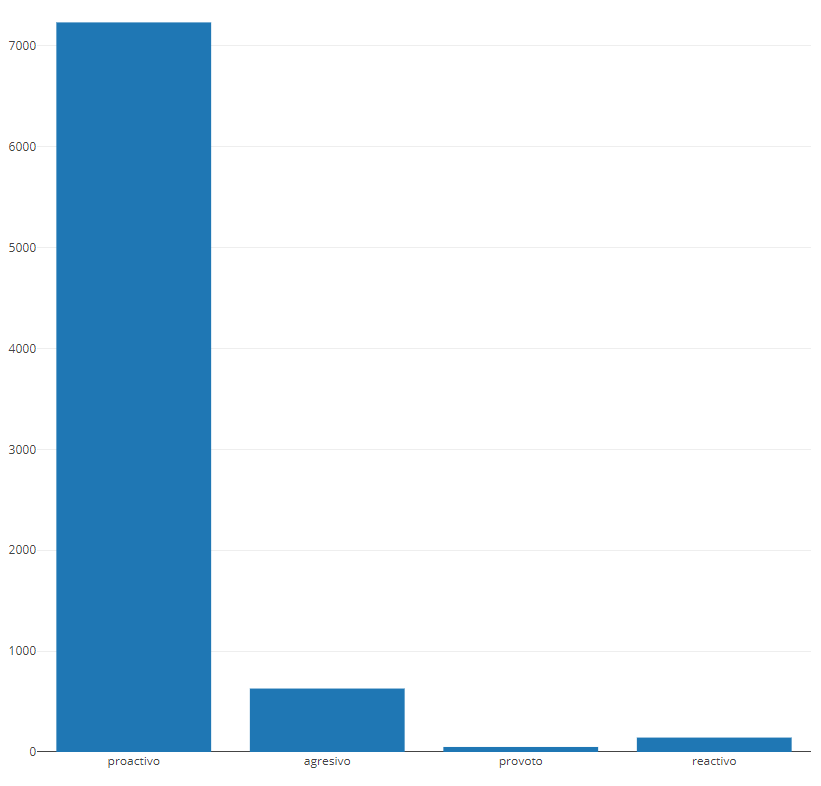
\includegraphics[width=2.80274in,height=2.68309in]{.//media/image2.png}



\end{minipage}

\caption{Data is heavily skewed towards proactive
attitude. The approach given in
\cref{proposed-algorithm} would help us ameliorate this
problem.}

\end{figure}



In most of the provided files there were three human annotators.
However, through a thorough database perusal it was found that only
Martha had valid annotations. So, let's do a variance analysis over each
of the target classes at least for Martha.



\begin{figure}[H]

\label{fig:commontasks}

\centering

\begin{minipage}{\textwidth}



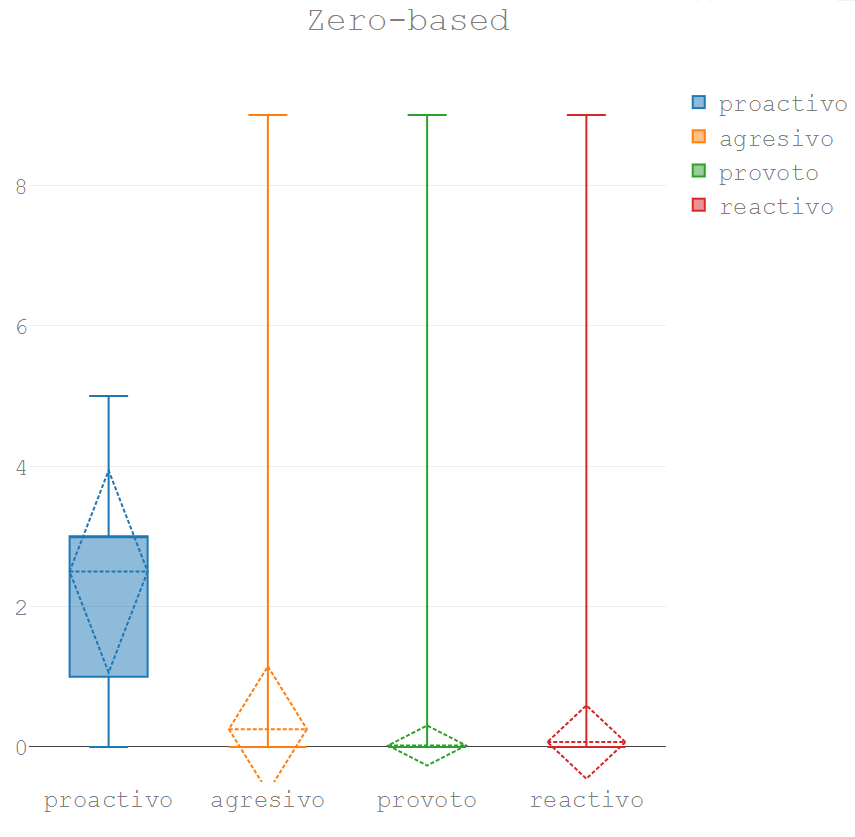
\includegraphics[width=2.77179in,height=2.71223in]{.//media/image3.png}



\end{minipage}

\caption{Overall category rankings provided by Martha}

\end{figure}



Just as expected, Martha is mostly filling the proactive field without
further care for any of the other categories. The rest of the categories
have a mean close to zero. However, a comparable variance analysis can
be done filtering out the times when those categories weren't used and
taking into account only the tweets which have a value greater than
zero.



\begin{figure}[H]

\label{fig:commontasks}

\centering

\begin{minipage}{\textwidth}



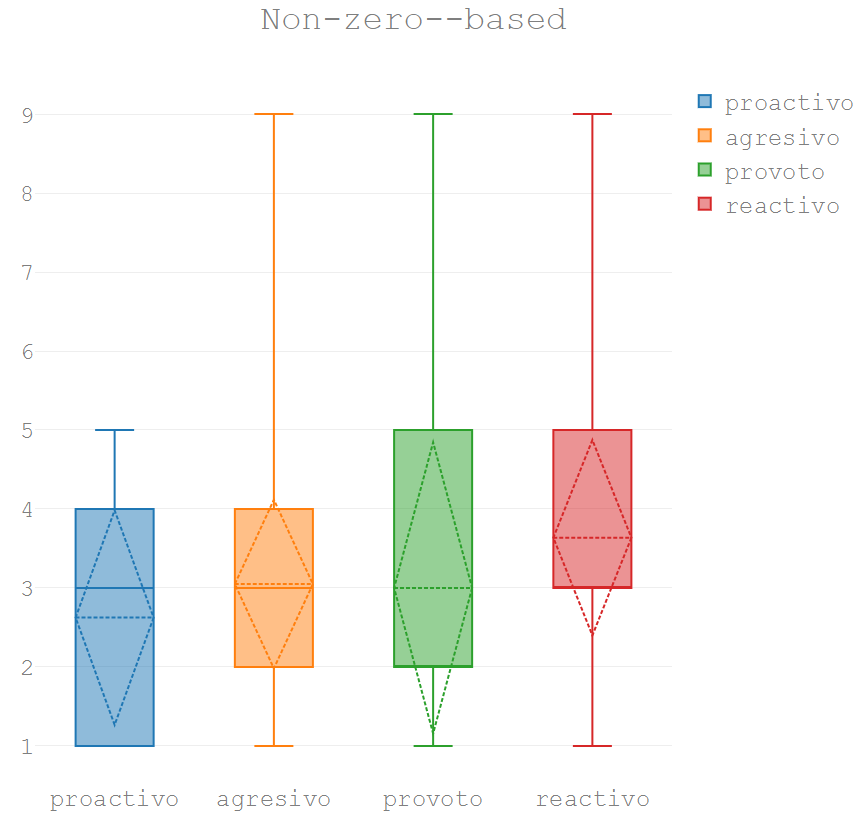
\includegraphics[width=2.95648in,height=2.87319in]{.//media/image4.png}



\end{minipage}

\caption{W hen Martha decides to use some category
($rank \neq 0$), which numbers she uses more
frequently}

\end{figure}



Here are some observations we can derive from the graph:

\begin{itemize}
\item
  While the most used category is proactive, Martha is still quite
  reserved in the scores she gave on this category, reaching a peak at
  5.
\item
  The vote-winner category has a similar interquartile range but reaches
  a more radical peak at 9.
\item
  The reactive and aggressive categories swing wildly but their means
  are between 3 and 4.
\end{itemize}

Now let's explore some the most common words that can serve of basis for
a bag-of-words representation. We will remove the stop words because
they are too common (low inverse document frequency) and do not add
value to the contrast we are trying to discover.



\begin{figure}[H]

\label{fig:commontasks}

\centering

\begin{minipage}{\textwidth}



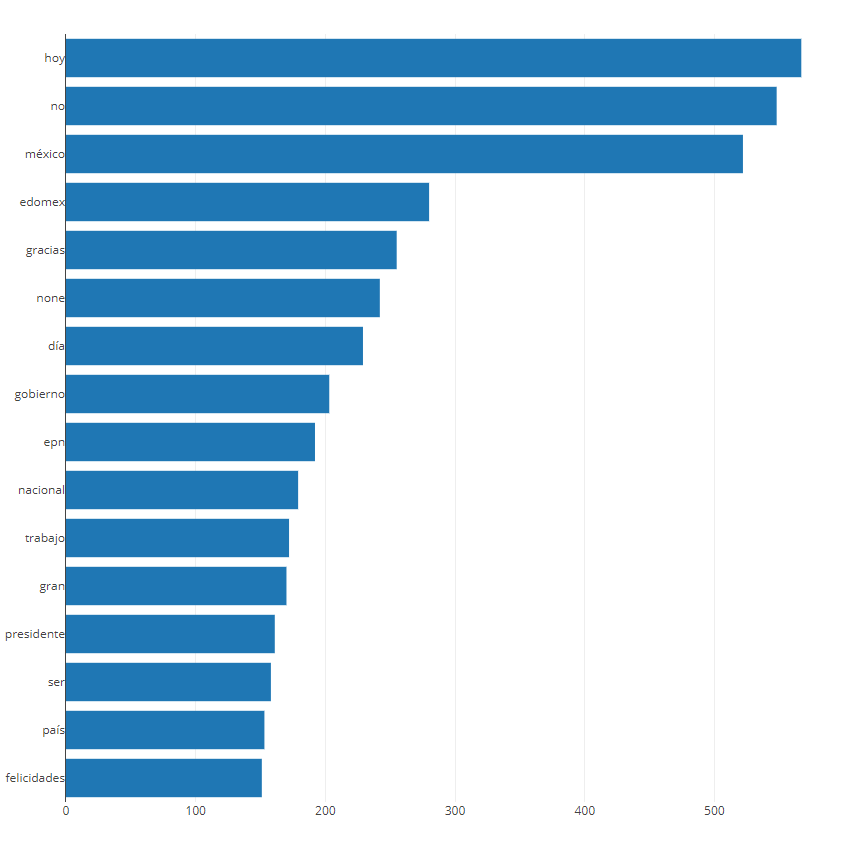
\includegraphics[width=3.97676in,height=3.98186in]{.//media/image5.png}



\end{minipage}

\caption{Bar chart showing the most frequent used word}

\end{figure}



However, this word list still contains political parties and names.
Let´s remove them and split by category usage.



\begin{figure}[H]

\label{fig:commontasks}

\centering

\begin{minipage}{\textwidth}



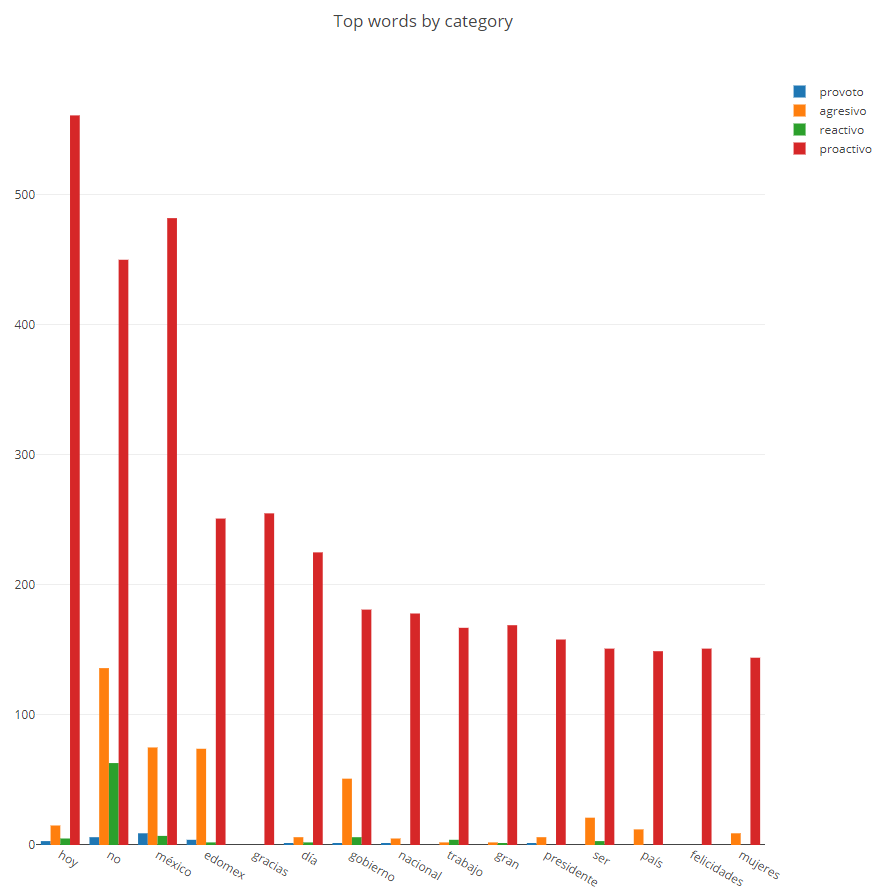
\includegraphics[width=2.84478in,height=2.89007in]{.//media/image6.png}



\end{minipage}

\caption{Most used words per category}

\end{figure}





\begin{figure}[H]

\label{fig:commontasks}

\centering

\begin{minipage}{\textwidth}



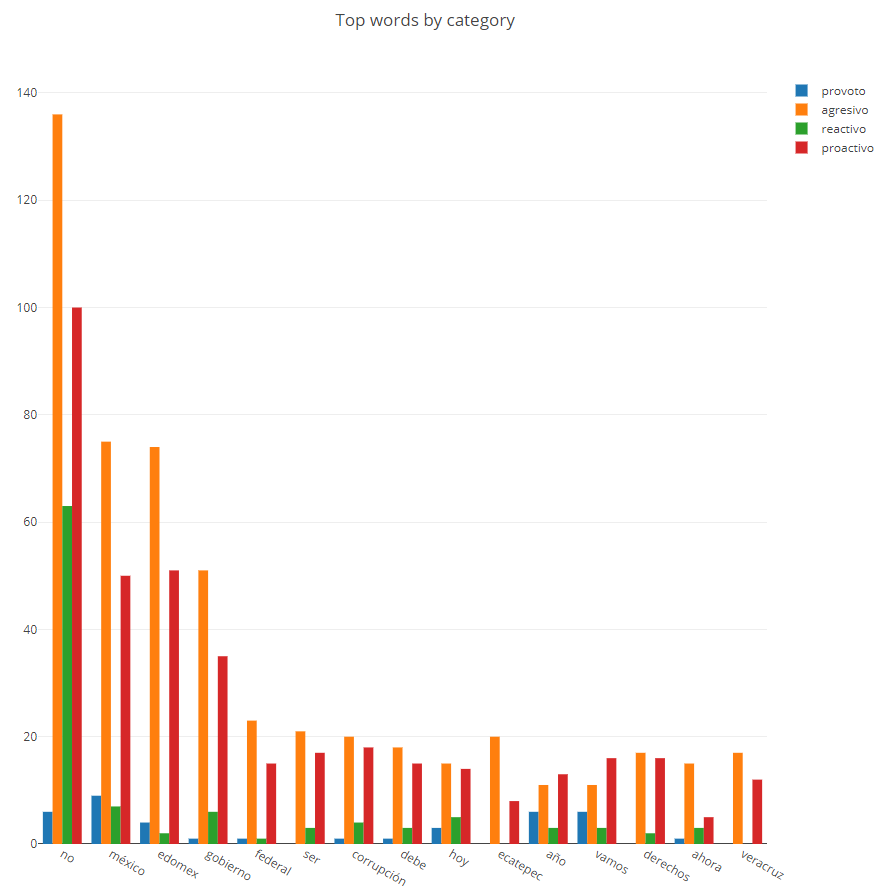
\includegraphics[width=2.69914in,height=2.72971in]{.//media/image7.png}



\end{minipage}

\caption{Word usage per category taking into account
that at least that word was used in other category from proactive }

\end{figure}



Owning to the fact that we added the word ``no'' to the exception list
is the most common word.

A ROC curve will be used to measure accuracy selecting different set of
features, once using a Naïve Bayes classifier and once using Random
Forest. Naïve Bayes classifiers works well when using prior binary
knowledge of which words are present in a sentence, even using a
bag-of-words and is probable it will get more uniform results. To
complete our test Random Forest will exploit the features more uniformly
and probably will get a significant improvement.

It is impossible to measure the statistical significance of the
improvement because we are only using one database. According to
\parencite{12011}
we need at least $n\eq a*
k$ where
$a$ is a
number between 2 and 8 and
$k$ is
the number of classifiers we are testing. Wilcoxon test, which deals for
just two classifiers as in our case, also relies on this number of
separate databases.

Finally, we are going to measure feature importance in the accuracy of
each classifier.

\section{Results and discussion}\label{results-and-discussion}

From a source code view (PyCharm project provided), the process taken to
generate the results where:

\begin{enumerate}
\def\labelenumi{\arabic{enumi}.}
\item
  In the \emph{cleansing} python package run the files in the following
  order:

  \begin{enumerate}
  \def\labelenumii{\alph{enumii}.}
  \item
    \textbf{Load\_tweets.py}. Centralizes the information contained in
    the provided Excels files into a one hdf5 and then a pickle file
    called final.pickle.
  \item
    \textbf{Tockenize\_tweets.py}. Generates the column
    \emph{tokenized\_text} which is the text array in which has cleansed
    text for the BOW extraction.
  \item
    \textbf{Generate\_tokenized\_text\_noparties.py}. Removes stopwords
    and political party names from the \emph{tokenized\_text} column.
  \item
    \textbf{Categories\_boxplot.py}. Visualize Martha preference
    treating the classes as if they were numerical.
  \end{enumerate}
\item
  The \emph{testing} package has some files we can use at this point.
  Those are:

  \begin{enumerate}
  \def\labelenumii{\alph{enumii}.}
  \item
    \textbf{Wordlist\_histogram.py}. Plot that shows the most frequent
    words that will be pprobably important for our classifier.
  \item
    \textbf{Wordlist\_category\_histogram.py}. Help us visualize the
    problem in terms of most frequent words distribution over the 4
    attitudes.
  \item
    \textbf{Box\_plots.py}. Visualize Martha preference contrasting
    attribute usage by the presence of zero.
  \end{enumerate}
\item
  Here comes our contribution. In the \emph{features} packages there are
  the following files:

  \begin{enumerate}
  \def\labelenumii{\alph{enumii}.}
  \item
    \textbf{ExtractBOW.py}. Binary bag-of-words vector extraction. All
    the extracted features are saved in Excel and pickle for latter
    usage.
  \item
    \textbf{SpecialTockens.py}. This file contain the function that we
    are going to evaluate in order to compute the special tokens ngram
    model.
  \item
    \textbf{ExtractBIG.py}. Common sense features are extracted first by
    counting special tokens. Then bigrams are extracted and counted to
    preserve grammatical structures that are obviated by the W2V
    representation.
  \item
    \textbf{ExtractW2V.py}. Spanish word2vec vector representation are
    extracted for each word and then and an average overall tweet vector
    is calculated.
  \item
    \textbf{ExtractFeatures.py}. Consolidate all the features into one
    file.
  \item
    \textbf{Save.py}. Save the features to an Excel and a Pickle file
    for rapid usage.
  \end{enumerate}
\item
  Having generated all the features, lets go back to our \emph{testing}
  package:

  \begin{enumerate}
  \def\labelenumii{\alph{enumii}.}
  \item
    \textbf{Test\_classifier.py} . Contains base functions for
    calculating the \emph{ROC AUC} for multiclass environment, as well
    as \textbf{precision}, \textbf{recall}, \textbf{accuracy} and
    \textbf{f1-scores} that can be appreciated indirectly on the
    confusion matrices. For the sake of conciseness, the only metric
    presented on the report was the \emph{ROC AUC}. A cross validation
    function is provided.
  \item
    \textbf{Confusion\_matrix.py}. Two graph type were generated, the
    general one presented on
    \Cref{generalresults}
    and the confusion matrices that will be explained in due course.
  \item
    \textbf{Feature\_importance.py}. Finally this file help us visualize
    what are the most relevant top 20 features for the \emph{W2V+BIG+BOW
    RandomForest}.
  \end{enumerate}
\end{enumerate}

Having explored the data we saw there is a tendency for proactive
classification. Thus, we should expect having low recall values for the
aggressive, vote-winner and reactive classes. Two classifiers will be
tested, a Naïve Bayes classifier that adapts very well to binary
features and a Random-Forest one that can use features more uniformly.
Both are natively multiclass. Random Forest was trained with 100 trees.

In this section we evaluate each of the feature sets individually taking
into account also the class there are trying to predict.



\begin{figure}[H]

\label{generalresults}

\centering

\begin{minipage}{\textwidth}



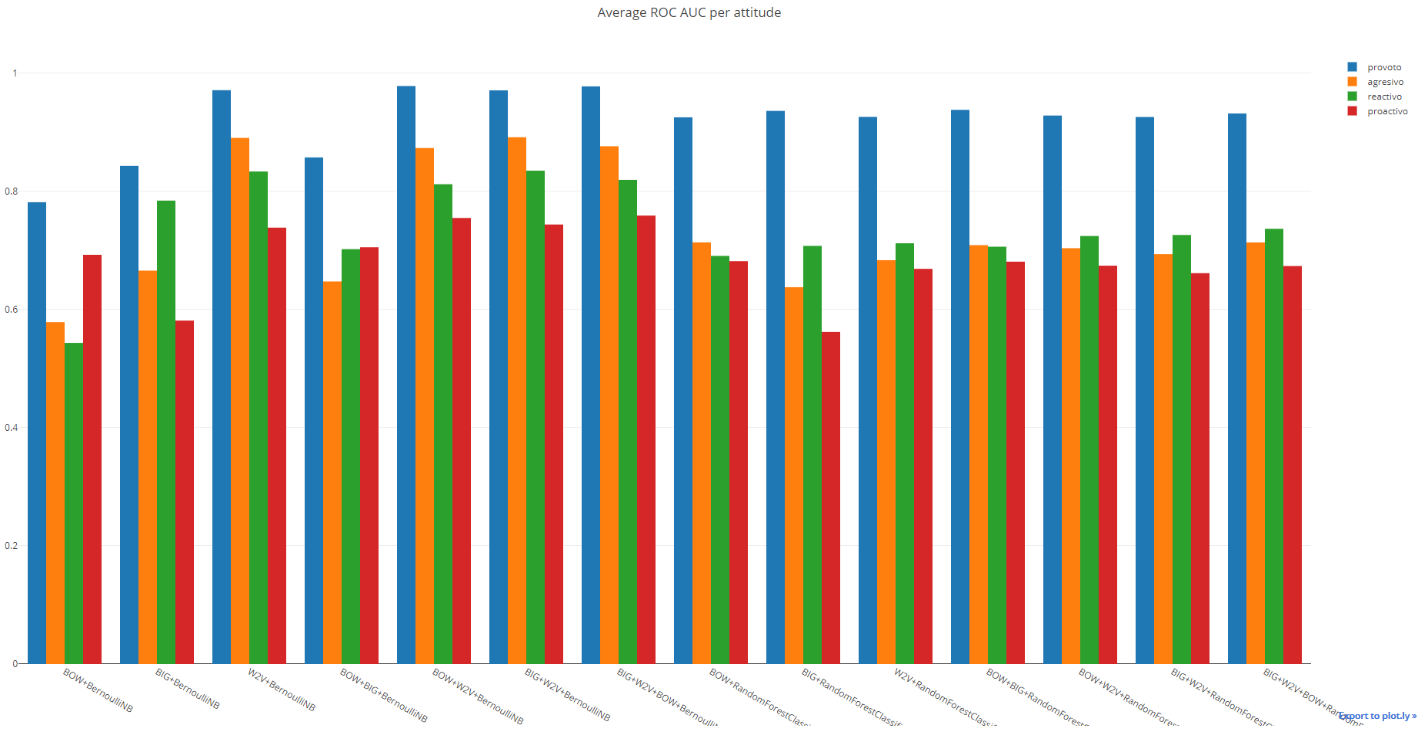
\includegraphics[width=6.49583in,height=3.32153in]{.//media/image8.png}



\end{minipage}

\caption{Results obtained expressed as the macro average
ROC area using a one vs rest classifier (Weka approach)}

\end{figure}



General ROC areas (one vs rest) demonstrate that BIG+W2V using Naïve
Bayes has a slightly better accuracy than the rest of the features. BOW
features actually worsened the classifier accuracy and so do using
Random Forest. However, literature recommends using confusion matrices
for measuring performance on multiclass classifiers. Let's derive some
conclusions from looking them.

\subsection{Bag-of-Words}\label{bag-of-words}

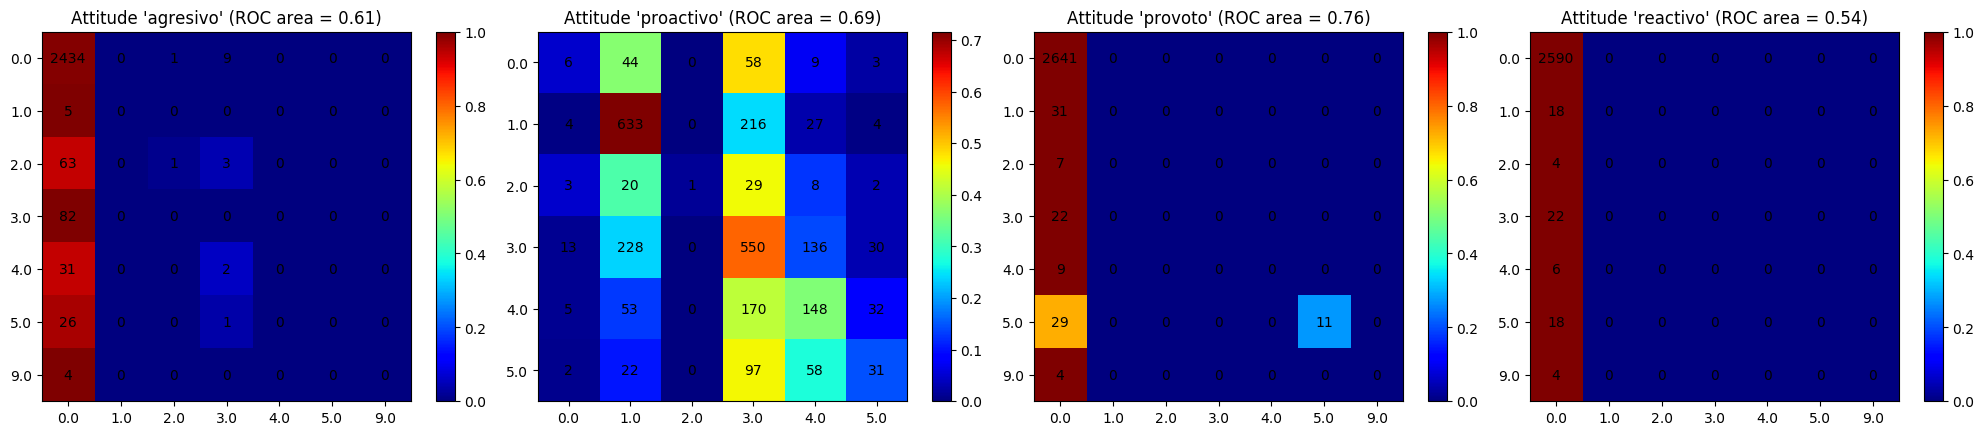
\includegraphics[width=6.48681in,height=1.42639in]{.//media/image9.png}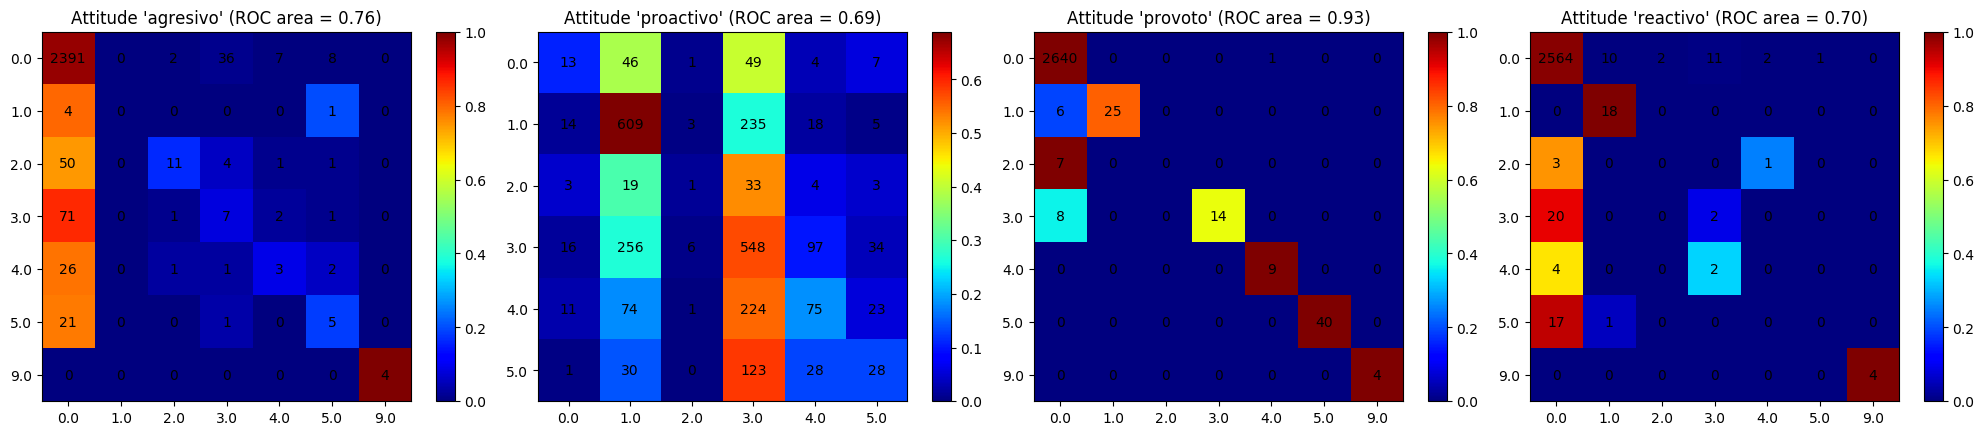
\includegraphics[width=6.48681in,height=1.42639in]{.//media/image10.png}

The first row of the confusion matrix heatmap show the BernoulliNB
classifier and the second one the RandomForestClassifier.

It is no surprise that bag-of-word has an good performance on the
\emph{Proactive} label. However, the actual data has a penchant for 3 so
our classifier fails to pickup this static tendency. \emph{Vote winner}
category improves significantly when we use maybe owning to the fact
that RandomForest uses the features better.

\subsection{Bigrams}\label{bigrams}

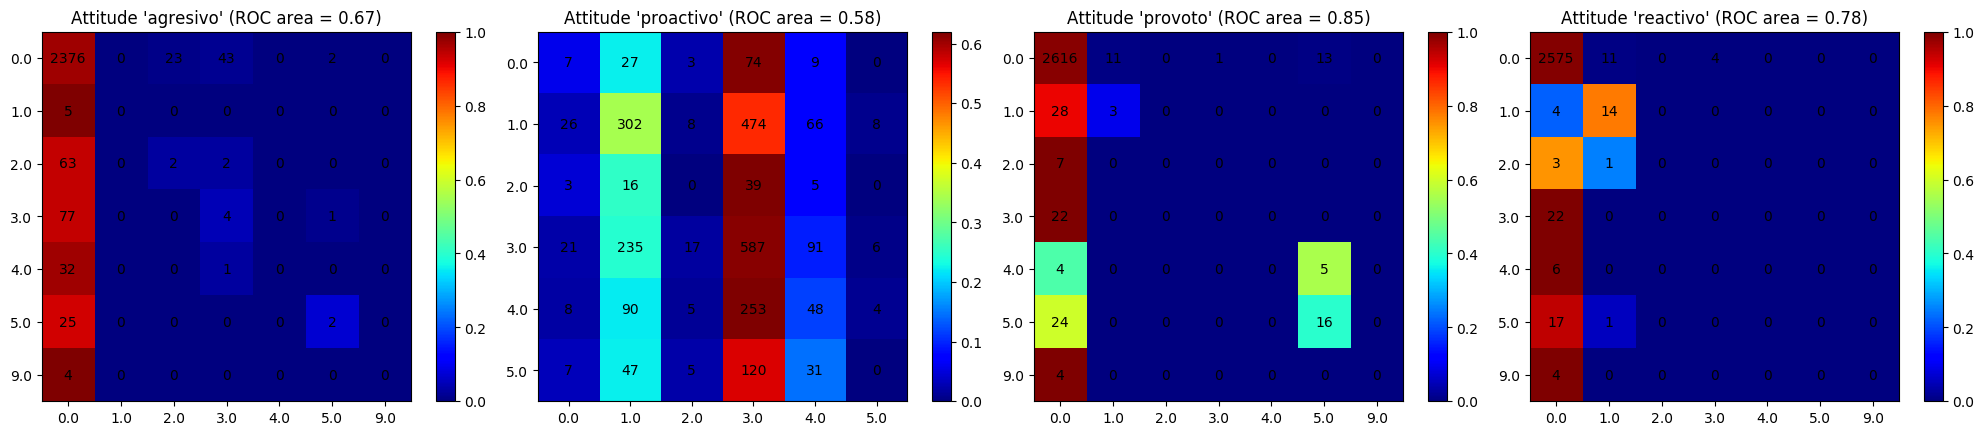
\includegraphics[width=6.48681in,height=1.42639in]{.//media/image11.png}

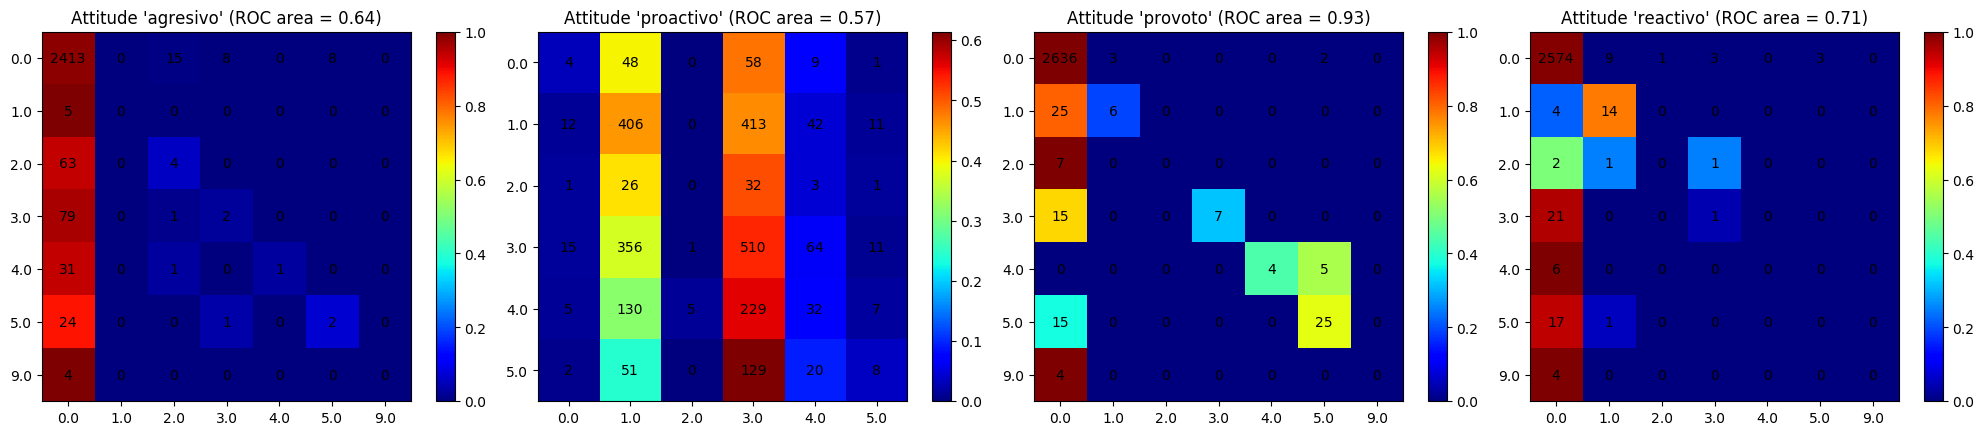
\includegraphics[width=6.48681in,height=1.42639in]{.//media/image12.png}

Compared to BOW, Bigrams improve the aggressive and the provote and
reactive categories using \emph{Naïve Bayes}. However, using
\emph{Random Forest} the behavior is a little worse.

\subsection{Word2Vec}\label{word2vec}

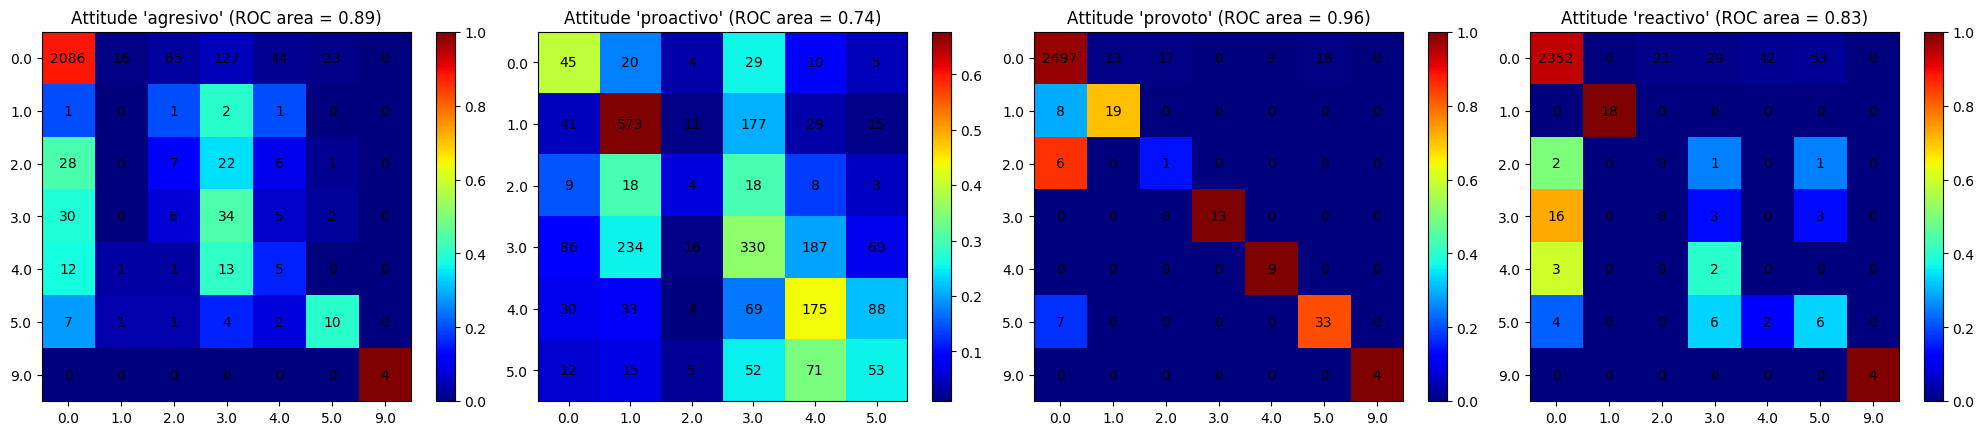
\includegraphics[width=6.48681in,height=1.42639in]{.//media/image13.png}

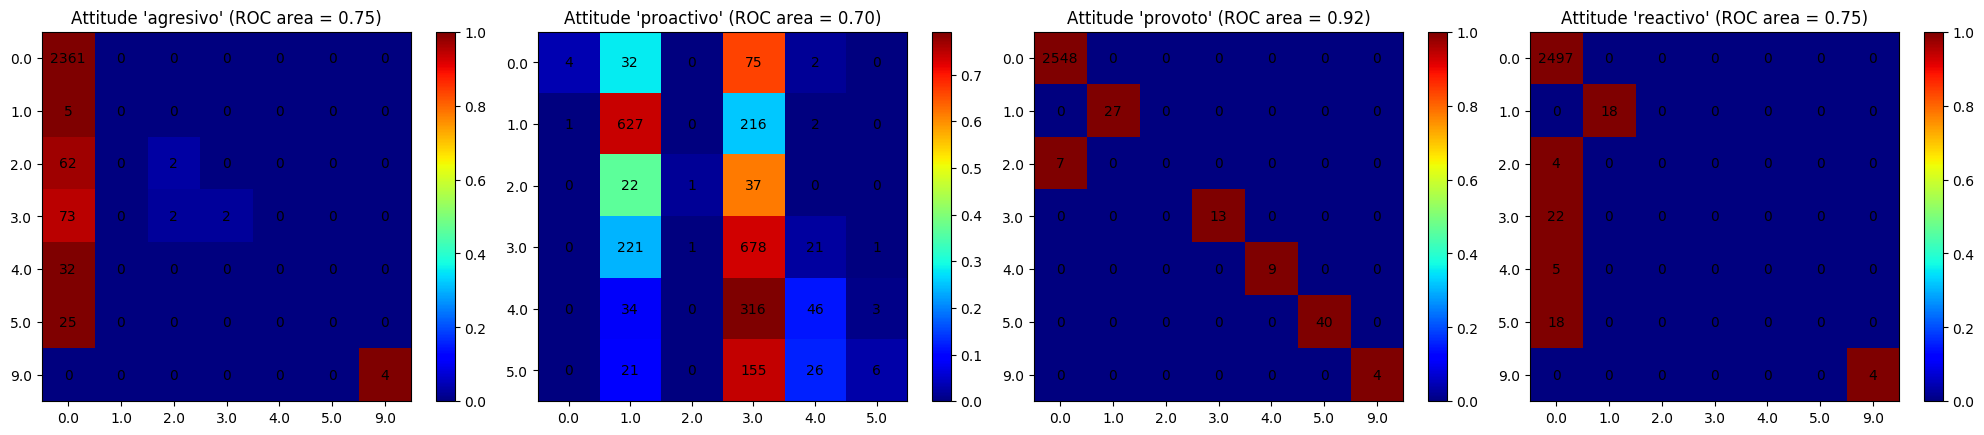
\includegraphics[width=6.48681in,height=1.42639in]{.//media/image14.png}

\emph{Word2vec} features improve substantially both NB and RF.
\emph{Provoto} precision and recall levels also seem to improve.

\subsection{Word2Vec + BOW}\label{word2vec-bow}

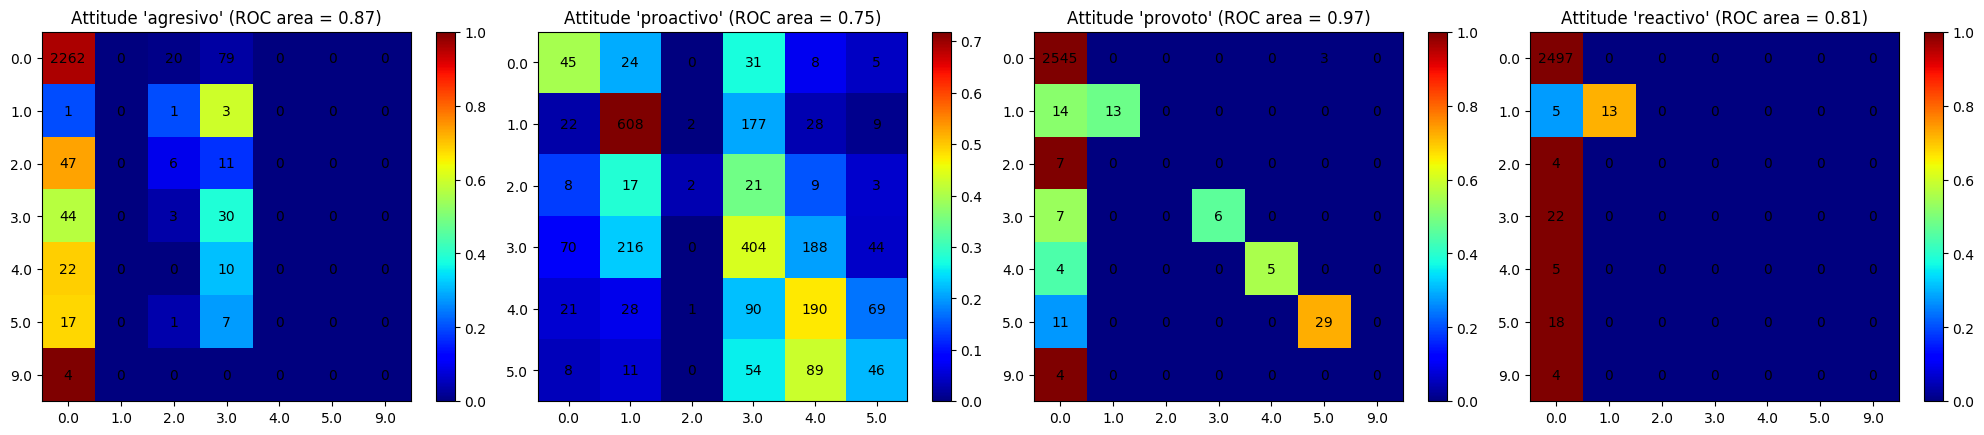
\includegraphics[width=6.48681in,height=1.42639in]{.//media/image15.png}

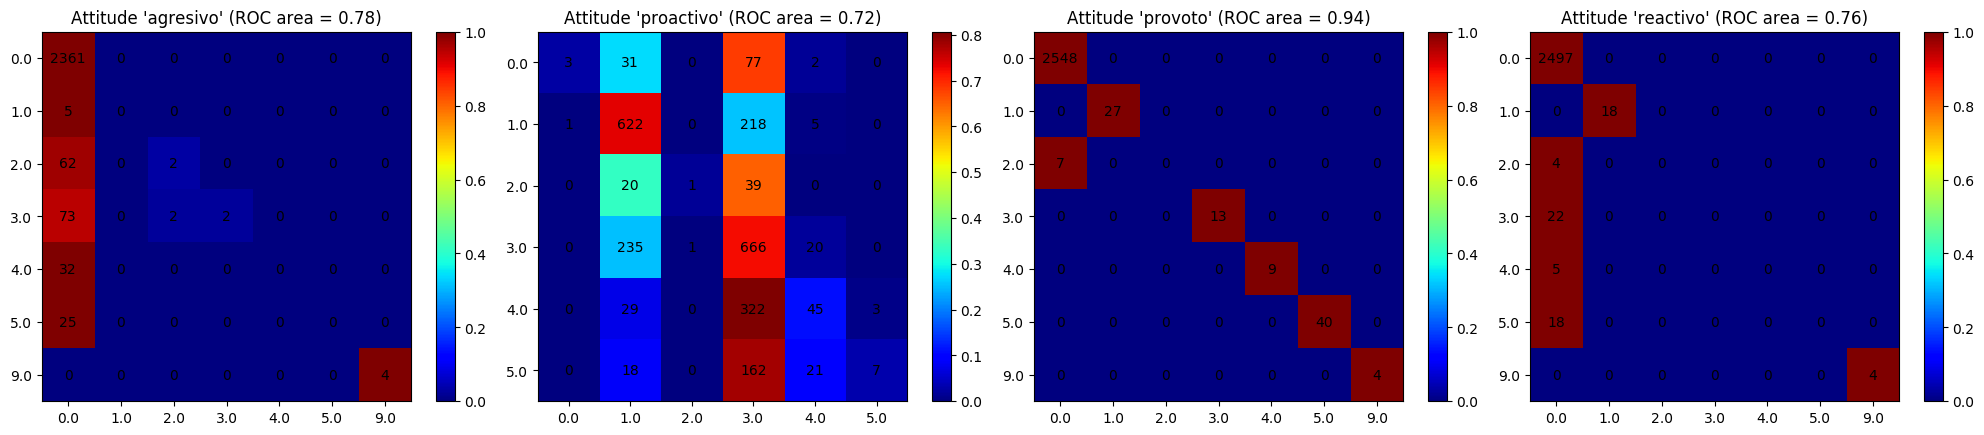
\includegraphics[width=6.48681in,height=1.42639in]{.//media/image16.png}

\subsection{Word2Vec + Bigrams}\label{word2vec-bigrams}

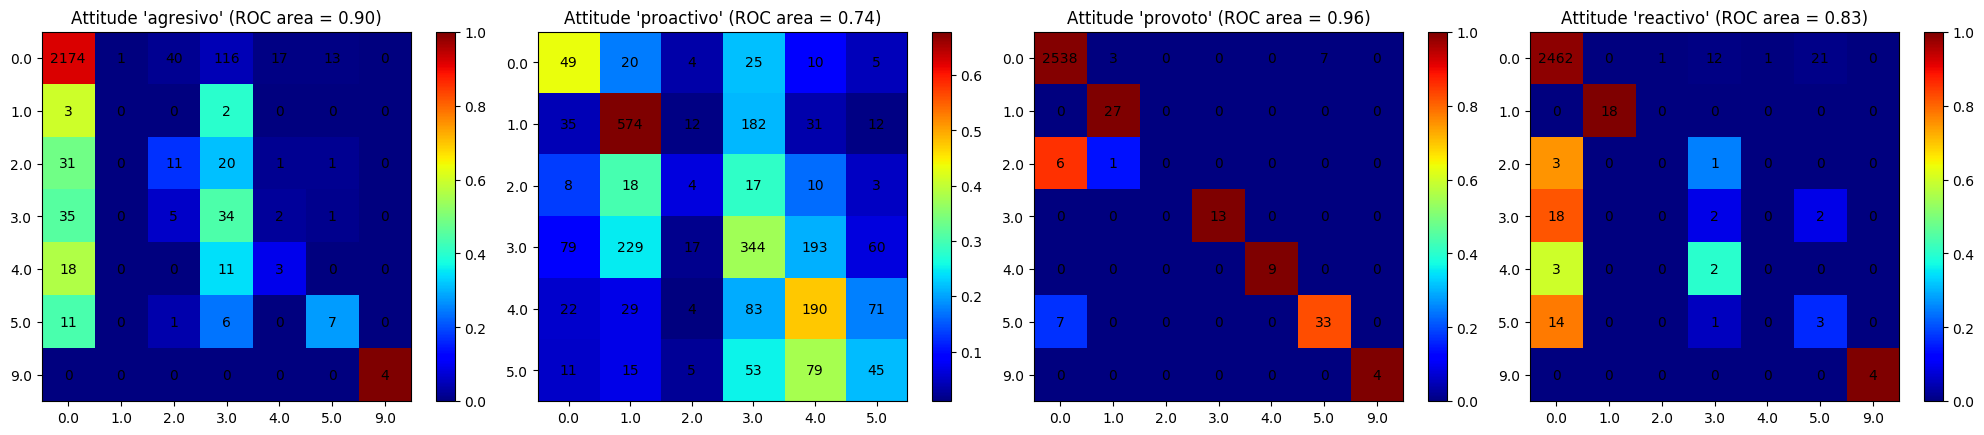
\includegraphics[width=6.48681in,height=1.42639in]{.//media/image17.png}

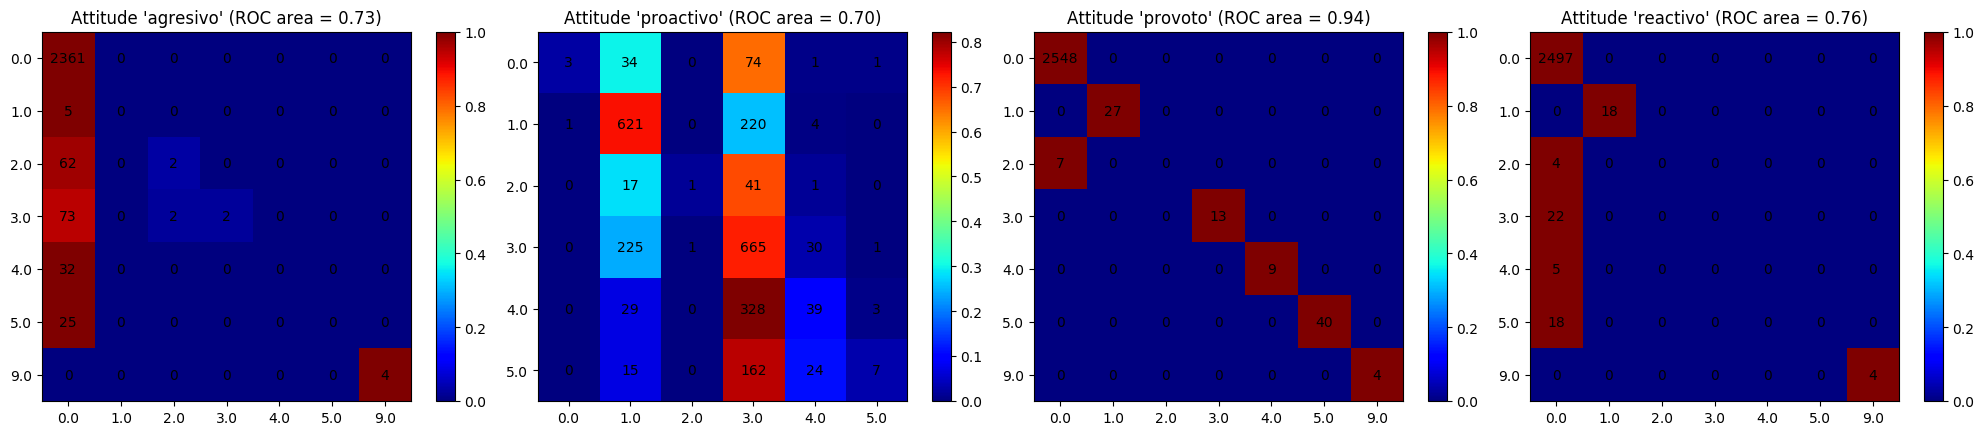
\includegraphics[width=6.48681in,height=1.42639in]{.//media/image18.png}

\subsection{BOW + Bigrams}\label{bow-bigrams}

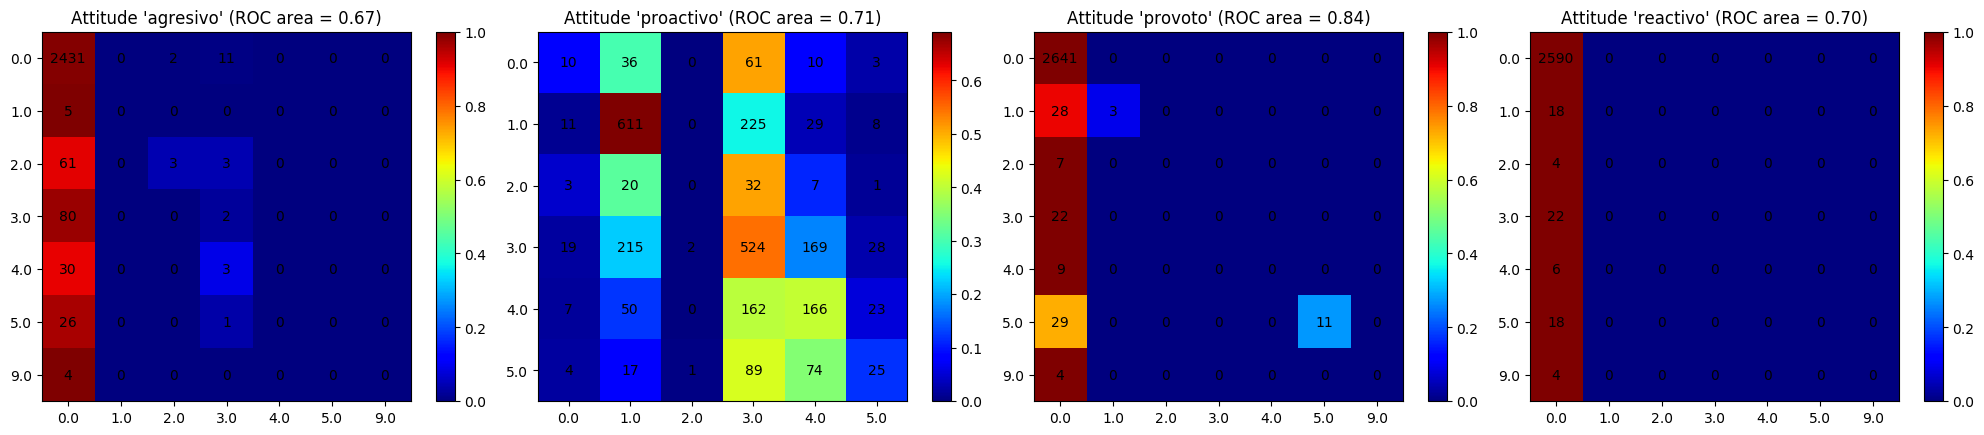
\includegraphics[width=6.48681in,height=1.42639in]{.//media/image19.png}

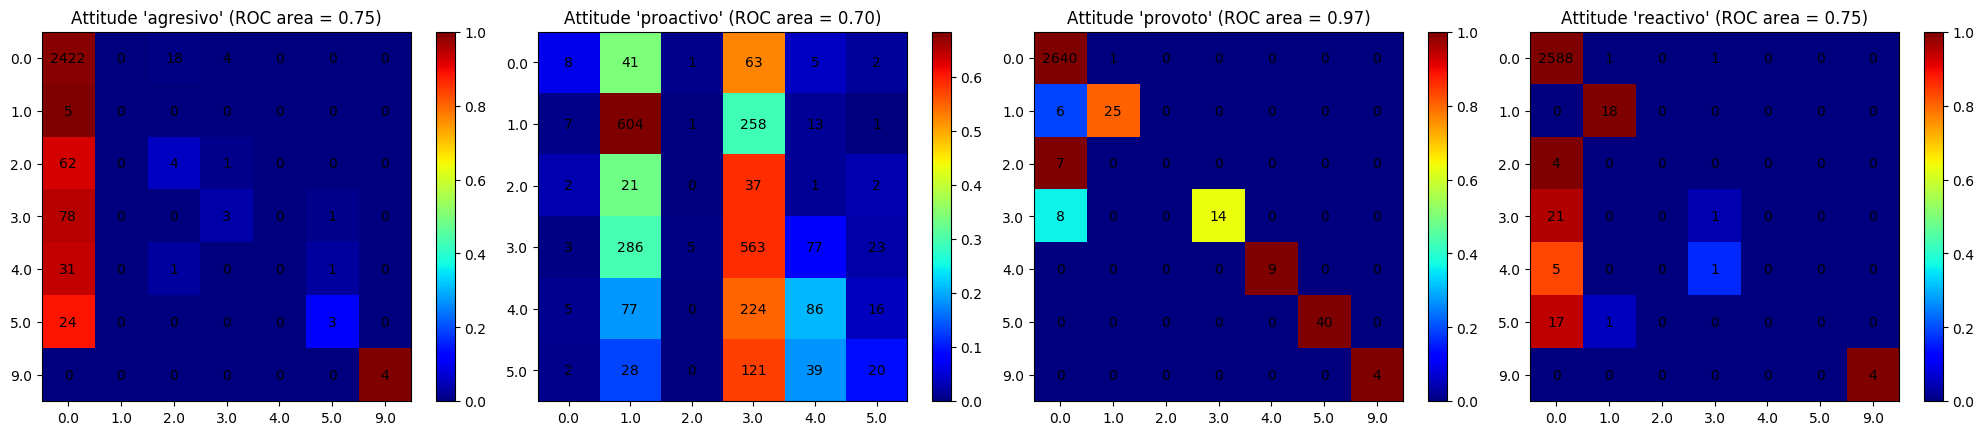
\includegraphics[width=6.48681in,height=1.42639in]{.//media/image20.png}

Mixed features (BOW + W2V + BIG)

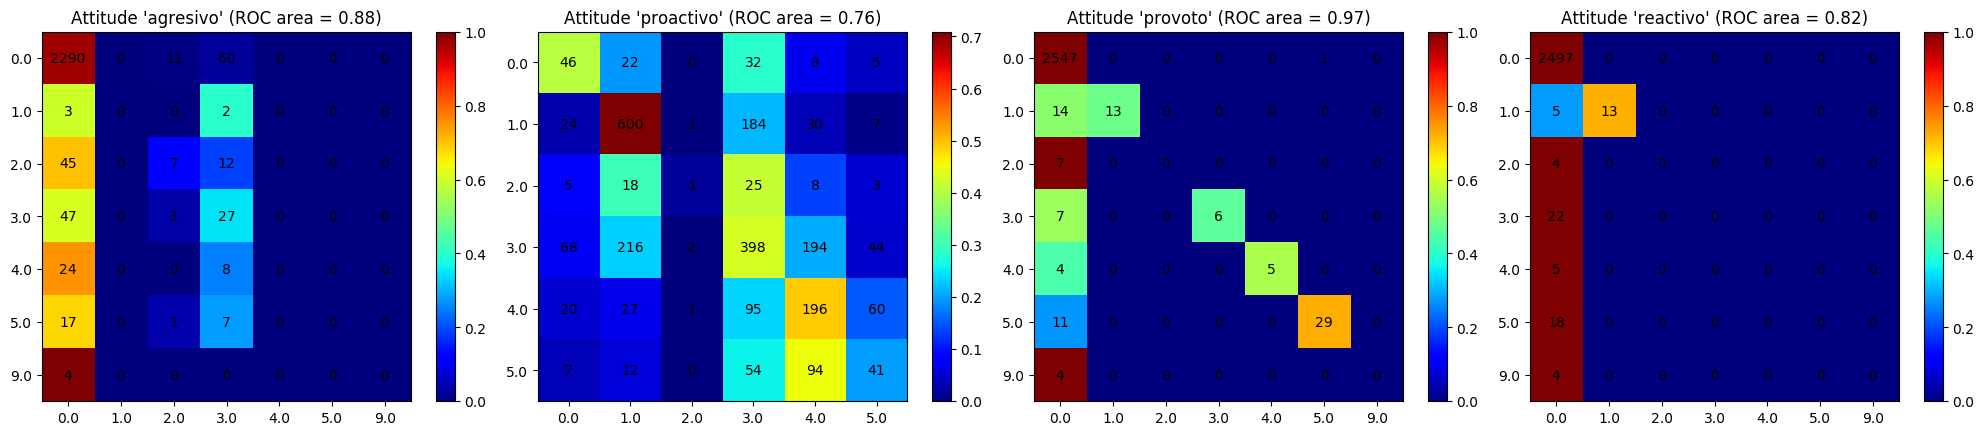
\includegraphics[width=6.48681in,height=1.42639in]{.//media/image21.png}

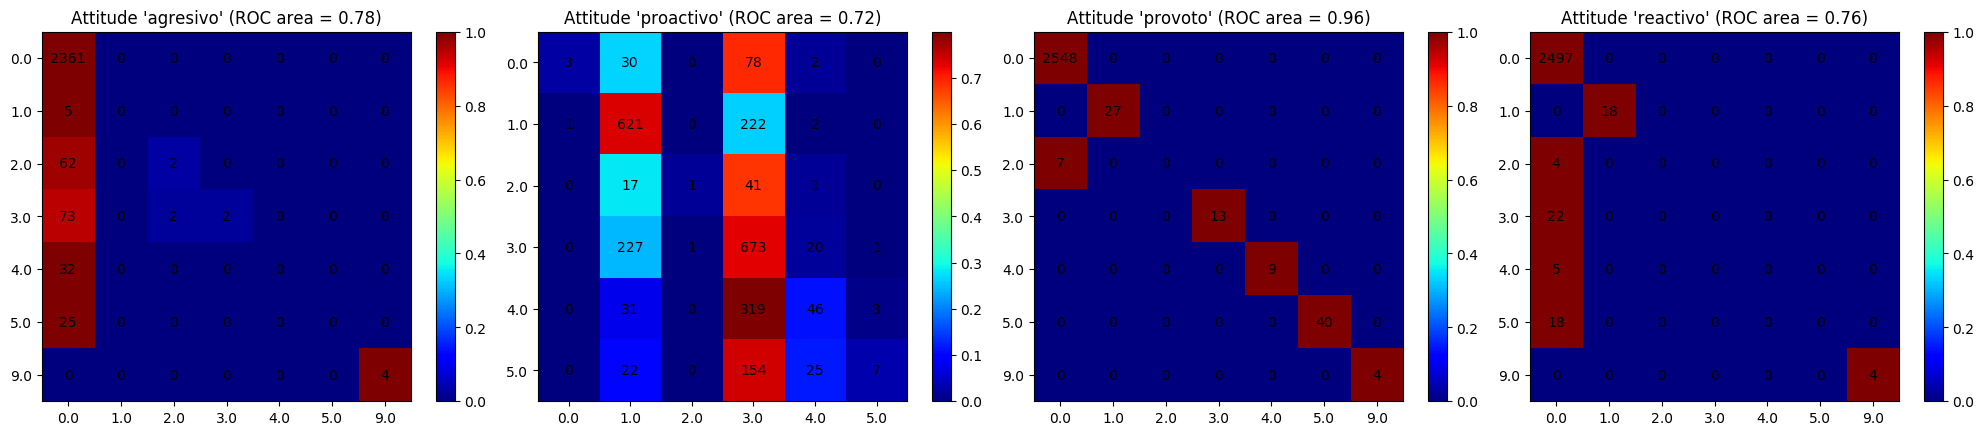
\includegraphics[width=6.48681in,height=1.42639in]{.//media/image22.png}

All the features combine generate a nearly perfect \emph{Provoto}
classification for \emph{RandomForest}. However, that is as far as it
gets, because the data is insufficient for learning other classes. The
vertical lines indicate that the actual class is always static, the
source of a big generalization error that could be ameliorated if we had
more data.

\section{Feature importance}\label{feature-importance}

We can see from the following figures that that most helpful features
come from the word2vec classifier. Some come from BIG and a bit fewer
from BOW.



\begin{figure}[H]

\label{generalresults}

\centering

\begin{minipage}{\textwidth}



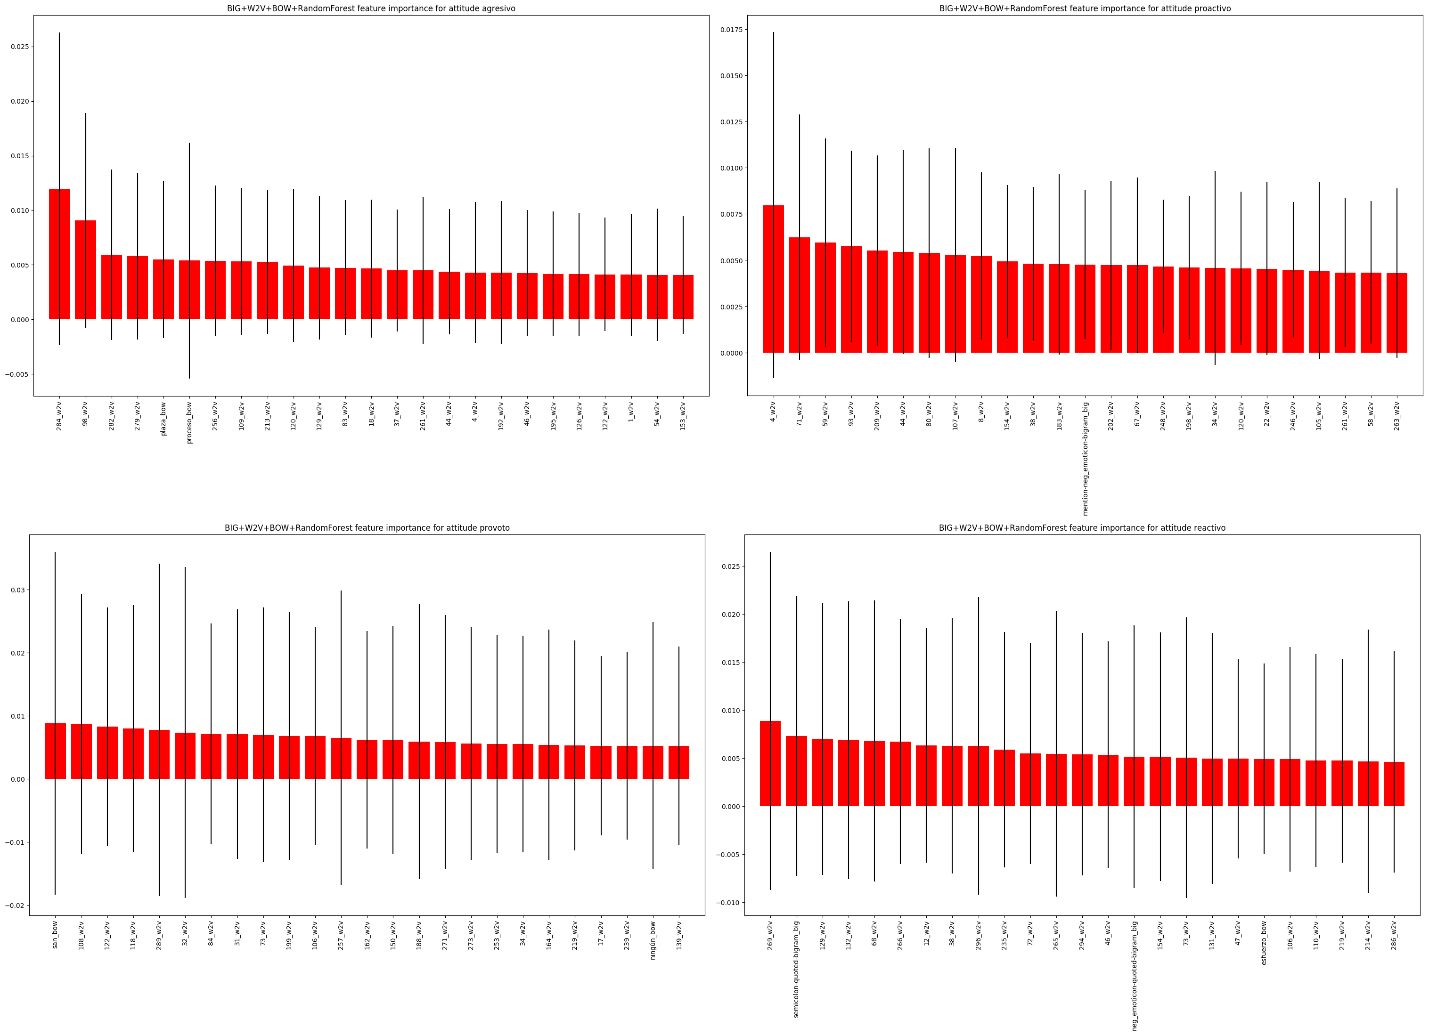
\includegraphics[width=6.49583in,height=4.70417in]{.//media/image23.png}



\end{minipage}

\caption{Feature importance}

\end{figure}



\section{Conclusions}\label{conclusions}

Features with which we feed a machine learning algorithm are very
important. We just saw how by just adding bigram features improved
accuracy and \emph{ROC AUC} consistently. Feature work may generate more
levels of bigrams and then made feature extraction by importance to
improve the \emph{recall} of the classifier.

Word2vec vector representation can help integrate the syntactic and
semantic structures of any language and find similarities between
sentences. Those similarities can then be used to train a more complex
classifier.

The vertical lines in our results indicate that the actual class is
static and that there is a big generalization error, so we probably we
could do better with more data.

\section{Reference work listing}\label{reference-work-listing}

An interesting study on political analysis of tweets was done by
\parencite{2017a}
in which a Spanish tweets were used in conjunction with word2vec for
political elections prediction. They measure their results over the
F1-score and using Support Vector Machines. On two distinct phases of
2242 and 16 million tweets, they achieved 60.5\% and 85.09\%
respectively. A similar approach of building n-grams was used. Compared
to our results they achieved better results but that can be explained by
the nature of their problem which was a single class problem.

Another starting point was the work published in
\parencite{2017b}.
However, in that work they don't use bigram generation nor bigram
counting to feed the classifiers.

\section{References}\label{references}





\bibliography{bib}



\end{document}


